\documentclass[12pt]{article}
\usepackage[a4paper,margin=1in]{geometry}
\usepackage[T1]{fontenc}
\usepackage[utf8]{inputenc}
\usepackage{lmodern}
\usepackage{amsmath,amssymb}
\usepackage{booktabs}
\usepackage{float}
\usepackage{array}
\usepackage{longtable}
\usepackage{enumitem}
\usepackage{xcolor}
\usepackage{graphicx}
\usepackage{listings}
\usepackage{microtype}
\usepackage{hyperref}
\hypersetup{colorlinks=true, urlcolor=blue, linkcolor=blue}

\setlength{\parindent}{0pt}
\setlength{\parskip}{0.75\baselineskip}
\setlist{nosep,leftmargin=*}
\renewcommand{\arraystretch}{1.25}


\lstdefinelanguage{json}{
    basicstyle=\ttfamily\small,
    showstringspaces=false,
    breaklines=true,
    morestring=[b]",
    stringstyle=\color{black},
    morekeywords={true,false,null},
    keywordstyle=\color{black}
}

\lstset{
    basicstyle=\ttfamily\small,
    breaklines=true,
    frame=single,
    columns=fullflexible,
    keepspaces=true,
    showstringspaces=false
}

\begin{document}

\begin{titlepage}
    \centering
    % University and Faculty Information
    {\large \textbf{HANOI UNIVERSITY OF SCIENCE AND TECHNOLOGY}} \\[0.5cm]
    
    
    % Course Information
    {\large \textbf{School of Information and Communications Technology}} \\
    \vspace{1.0cm}

    {\includegraphics[width=0.3\textwidth]{logo.jpg}\\}
    \vspace{1.0cm}
    % Project Title
    \rule{\textwidth}{1pt}\\[0.5cm]
    {\Large \textbf{Probabilistic Atmospheric Spectrum Retrieval}}\\[0.2cm]
    {\Large \textbf{for the Ariel Data Challenge 2025}}\\[0.4cm]
    {\textbf{A Physics-Based Machine Learning Pipeline with Uncertainty Calibration}}\\[0.2cm]
    \rule{\textwidth}{1pt}\\[1cm]
    
    \textbf{Lecturer: Dr. Dam Quang Tuan}

    \textbf{Group 8 - Class 168272}
    
    \begin{tabular}{ll}
        \textbf{Pham Tien Dung} & 202416680\\
        \textbf{Tran Nam Hai} & 202400103\\
        \textbf{Nguyen Vu Trung Kien} & 202416713\\
        \textbf{Nguyen Duc Hoai Anh} & 202416662 \\
        \textbf{Nguyen Duc Minh} & 202416722 \\
    \end{tabular}
    
    \vfill
    
    {\large Hanoi, \the\year}
\end{titlepage}

\clearpage
\tableofcontents
\clearpage

\section{Abstract}

Recovering an exoplanet's atmospheric transmission spectrum - along with calibrated per-wavelength uncertainties - from raw telescope detector data is a challenging probabilistic regression problem: the transit signal is faint ($\sim$0.1-2\% of stellar flux), instrument noise is heteroscedastic across wavelengths, and the official evaluation metric (normalised Gaussian Log-Likelihood, GLL) jointly penalises prediction error and mis-calibrated confidence. We address this via the \href{https://www.kaggle.com/competitions/ariel-data-challenge-2025}{Ariel Data Challenge 2025} (NeurIPS), developing a physics-informed end-to-end pipeline and benchmarking 22 models across 7 families under identical cross-validation folds; we additionally formalise \textbf{PHC} (Physics-conditioned Heteroscedastic Calibration), a closed-form per-wavelength GLL-optimal uncertainty rescaling, and evaluate six deep sequence architectures as baselines. Under a protocol-synchronised comparison, tree ensembles achieve the best GLL score (Extra Trees 0.287, Random Forest 0.273), outperforming deep CNN/Transformer ($\sim$0.22); critically, uncertainty quality - not point-prediction accuracy - determines success, as XGBoost's best-RMSE model scores GLL\,$=$\,0 due to uninformative uncertainty, and PHC proves empirically marginal since intrinsic model uncertainty is already adequate. These results establish that physics-based noise features and well-calibrated probabilistic outputs are the dominant levers for this task, and that valid ML-vs-Deep comparisons require strict protocol synchronisation.

\section{Introduction}

\subsection{Background and Motivation}

Transit spectroscopy is the primary technique for characterising exoplanetary atmospheres remotely: when a planet crosses in front of its host star, its atmosphere selectively absorbs starlight at specific wavelengths, imprinting a \textbf{wavelength-dependent transmission spectrum} onto the observed stellar flux. Decoding this spectrum reveals atmospheric composition and structure, but the signal is extremely faint - typically $\sim$0.1-2\% of stellar flux - and buried in instrumental and photon noise, making automated, uncertainty-aware retrieval a fundamental open challenge.

The ESA \emph{Ariel} mission addresses this at survey scale, targeting $\sim$1,000 exoplanets with two dedicated instruments: the \textbf{FGS1} visible-light photometer and the \textbf{AIRS-CH0} infrared spectrometer (283 wavelength channels, 1.95-3.90\,$\mu$m). The \href{https://www.kaggle.com/competitions/ariel-data-challenge-2025}{Ariel Data Challenge 2025} (NeurIPS) operationalises this retrieval problem as a supervised learning benchmark on simulated Ariel-like detector data. Crucially, the competition grades a \textbf{full predictive distribution} over each wavelength via a normalised \textbf{Gaussian Log-Likelihood (GLL)}, penalising both inaccurate means and mis-calibrated uncertainties equally. A model must therefore output a mean spectrum \textbf{and} a credible per-wavelength uncertainty - his is a genuine \emph{probabilistic regression} task where uncertainty quantification is a first-class objective, not an afterthought.

\textbf{Task.} Given noisy detector signals for a planet ($\sim$1,100 training planets), predict 283 spectral values $\mu_\lambda \approx (R_p/R_s)^2$ and 283 per-wavelength uncertainties $\sigma_\lambda$.

\subsection{Contributions}

\begin{enumerate}
\item \textbf{End-to-end physics-informed pipeline.} A full preprocessing stack - detector calibration $\rightarrow$ CDS light-curve extraction $\rightarrow$ transit detection $\rightarrow$ physics feature engineering $\rightarrow$ Target-PCA regression - implemented as a reusable, tested library (\texttt{src/}).

\item \textbf{Systematic 22-model benchmark.} Seven model families (linear, Bayesian, kernel/SVM, neighbours, tree ensembles, shallow neural, deep sequence) evaluated on the official GLL metric under identical GroupKFold cross-validation folds, enabling a fair, metric-faithful comparison.

\item \textbf{PHC uncertainty-calibration framework.} Physics-conditioned Heteroscedastic Calibration, with a closed-form per-wavelength GLL-optimal scale derived analytically. PHC standardises $\sigma$ across model families for the fair comparison in \S6.6; its empirical effect on the score is reported honestly as a \textbf{negative result}.

\item \textbf{Deep sequence baselines.} Six architectures (CNN1D, TCN, LSTM, GRU, Transformer, Autoencoder+MLP) trained end-to-end on calibrated light curves, with a $(\mu, \log\sigma)$ output head and Gaussian NLL loss.

\item \textbf{Protocol-synchronised ML-vs-Deep comparison.} Both model classes evaluated on the same held-out planets with the same PHC calibration and the same naive reference - the only valid basis for an ML-vs-Deep claim. Negative results (PHC marginal gain, mean/shape decomposition failure) are reported in full.
\end{enumerate}

\textit{Note on emphasis.} The primary contributions are the \textbf{systematic benchmark}, the \textbf{protocol-synchronised comparison}, and the \textbf{``uncertainty quality gates the score''} finding. PHC is a theoretically grounded analysis tool; it does not improve the score on this dataset, and we argue that reporting this honestly is itself a methodological contribution.
\section{Problem Formulation}

\subsection{Inputs and Outputs}

The competition provides two raw signal sources per planet, a set of calibration products, and stellar metadata. Table~\ref{tab:inputs} summarises each component and its role in the pipeline.

\begin{table}[H]
\centering\small
\caption{Input components and their roles.}
\label{tab:inputs}
\begin{tabular}{@{}p{0.28\linewidth} p{0.64\linewidth}@{}}
\toprule
\textbf{Component} & \textbf{Role} \\
\midrule
AIRS-CH0 signal & Infrared spectrometer; 3-D tensor \texttt{[time, spatial, wavelength]} - primary source of spectral information across 283 channels (1.95-3.90\,$\mu$m) \\
FGS1 signal & Visible-light photometer; high-SNR white-light light curve used for transit timing and shape \\
Calibration files & Dead-pixel map (\texttt{dead}), dark frame (\texttt{dark}), flat field (\texttt{flat}), linearity correction (\texttt{linear\_corr}) \\
ADC info & Per-channel gain and offset for raw-count to physical-unit conversion \\
Star/planet info & Stellar radius, mass, effective temperature, $\log g$, orbital period \\
\texttt{train.csv} & Ground-truth transmission spectra - 283 values per planet, target of regression \\
\bottomrule
\end{tabular}
\end{table}

Raw observations are stored as parquet files under \texttt{train/} and \texttt{test/}, grouped by \texttt{planet\_id}. Top-level metadata files include \texttt{train\_star\_info.csv}, \texttt{adc\_info.csv}, and \texttt{wavelengths.csv} (283 wavelength positions). All splits and joins are keyed by \texttt{planet\_id}.

\textbf{Output.} For each of the $\sim$1,100 training planets, predict $\boldsymbol{\mu} \in \mathbb{R}^{283}$ (mean transmission spectrum) and $\boldsymbol{\sigma} \in \mathbb{R}^{283}$ (per-wavelength uncertainty), where $\mu_\lambda \approx (R_p/R_s)^2$ is the squared planet-to-star radius ratio at wavelength $\lambda$.

\subsection{Evaluation Metric - Normalized Gaussian Log-Likelihood}

Each prediction $(\mu_\lambda, \sigma_\lambda)$ is interpreted as a Gaussian distribution over the ground-truth value $y_\lambda$. The per-element log-likelihood is

\[
\mathrm{GLL}(y,\mu,\sigma) = -\frac{1}{2}\!\left(\log(2\pi) + \log\sigma^{2} + \frac{(y-\mu)^2}{\sigma^2}\right),
\]

for each planet $i$ and wavelength $\lambda$. Each element is then normalised against two references:

\[
s_{i\lambda} = \frac{\mathrm{GLL}(y_{i\lambda},\,\mu_{i\lambda},\,\sigma_{i\lambda}) - \mathrm{GLL}(y_{i\lambda},\,\bar{\mu}_\lambda,\,\bar{\sigma}_\lambda)}{\mathrm{GLL}(y_{i\lambda},\,y_{i\lambda},\,\sigma^\star_\lambda) - \mathrm{GLL}(y_{i\lambda},\,\bar{\mu}_\lambda,\,\bar{\sigma}_\lambda)},
\]

where $(\bar{\mu}_\lambda, \bar{\sigma}_\lambda)$ are the training-set mean and standard deviation (naive reference), and $\sigma^\star_\lambda$ is an instrument-specific ideal uncertainty: $\sigma^\star = 1\,\text{ppm} = 10^{-6}$ for the FGS1 channel and $\sigma^\star = 10\,\text{ppm} = 10^{-5}$ for all AIRS-CH0 channels. The final score is the weighted average of all per-element scores, clipped to $[0, 1]$:

\[
\text{score} = \mathrm{clip}\!\left(\frac{\sum_{i,\lambda} w_\lambda\, s_{i\lambda}}{\sum_{i,\lambda} w_\lambda},\; 0,\; 1\right),
\]

where by default all channel weights $w_\lambda = 1$. A score of 0 means no better than naive; 1 means ideal.

\textbf{Why this metric is hard.} The GLL penalises two types of failure simultaneously: a large residual $(y - \mu)^2/\sigma^2$ punishes inaccurate means, while $\log\sigma^2$ punishes over-wide uncertainties. A model with accurate means but a mis-scaled $\sigma$ is still heavily penalised - this is why XGBoost (best RMSE) scores 0, and why uncertainty calibration is a first-class concern throughout this work.

\textbf{Baseline interpretation.} A score of 0 does not mean the model is useless - it means the joint mean-uncertainty likelihood is no better than predicting the training-set average for every planet. Models with low RMSE can and do score 0 if their uncertainty estimate is uninformative (too wide or too narrow).


\section{Background \& Related Work}

\subsection{Physics of transit spectroscopy}

For a transiting planet, the fractional dip in stellar flux at wavelength $\lambda$ equals the squared planet-to-star radius ratio,
\[
d_\lambda = 1 - \frac{\text{flux}_{\text{in}}}{\text{flux}_{\text{out}}} \approx \left(\frac{R_p}{R_s}\right)^2,
\]
and the \textbf{wavelength dependence} of $d_\lambda$ encodes the atmospheric composition: molecules absorb at characteristic wavelengths, making the planet appear slightly larger at those wavelengths. Transit depth is therefore the single most informative quantity, and the retrieval task reduces to estimating per-wavelength depths from noisy, time-series detector data.

Traditional atmospheric retrievals use Bayesian inference (MCMC or nested sampling) paired with physically motivated forward models to obtain full posterior distributions over atmospheric parameters. While principled, these methods require hours to days per planet and cannot scale to surveys of $\sim$1,000 targets - motivating the shift to machine learning surrogates that trade full posteriors for fast, calibrated point predictions with uncertainties.

\subsection{Machine learning for Ariel-style retrieval}

The Ariel Machine Learning Data Challenge series (since 2019) has systematically explored ML approaches for this problem. Several findings from the literature directly inform our design.

\textbf{Physics-based preprocessing dominates over model complexity.} The NeurIPS 2024 Ariel Data Challenge overview paper (Mugnai et al., arXiv:2505.08940) reports that top solutions share a common recipe: heavy signal processing (binning, geometric correction, detrending) feeding simple, well-regularised regressors. One competitive team used signal binning with 5-30 spectral bins and bagging of 50 Ridge regression models, achieving 66.4\% GLL on cross-validation. Their finding that linear models extrapolate better than tree ensembles under the out-of-distribution test distribution is a useful counterpoint to our own result that tree ensembles win under a synchronised evaluation.

\textbf{Uncertainty quantification is a first-class objective.} Forestano et al. (arXiv:2508.04982) systematically compare PLS, SVM, KNN, Random Forest, XGBoost, and stacking ensembles for exoplanet retrieval from transmission spectra, finding that heteroscedastic uncertainty modelling consistently outperforms fixed-variance assumptions on GLL-style metrics. This directly motivates our PHC calibration framework.

\textbf{Transformer-based acceleration of Bayesian retrieval.} Exoformer (Pagliaro et al., arXiv:2603.27623) uses a transformer to generate informative priors for nested-sampling retrievals, achieving 3-8$\times$ speedup without loss of accuracy relative to classical MCMC. While not directly comparable to our regression setting, it establishes the viability of attention-based sequence models for spectral retrieval - consistent with our Transformer baseline ranking among the top deep models.

\textbf{Dataset shift is a known risk.} The official Ariel simulated dataset (Mugnai et al., arXiv:2605.03719) explicitly flags that ML models face ``dataset shift when observed distributions diverge from those of the training set'' - a risk materialised in our competition by the out-of-distribution test set (planets around unseen stellar types).

\subsection{Our design philosophy}

Our approach follows the established recipe - physics-based preprocessing, uncertainty as a first-class output, deep models as baselines rather than primary solutions - while extending it with (i) a systematic 22-model benchmark under the official metric, (ii) PHC as a principled uncertainty standardisation framework, and (iii) a protocol-synchronised ML-vs-Deep comparison that corrects for the evaluation confounds we identified in the merged benchmark.


\section{Data \& Exploratory Analysis}

We analyse the training targets ($\sim$1,100 planets $\times$ 283 wavelengths), the stellar and orbital metadata, and representative calibrated light curves. Cross-validation throughout uses \textbf{GroupKFold by planet} so the same planet never appears in both train and validation folds.

\subsection{The target is nearly rank-1}

\begin{figure}[H]
\centering
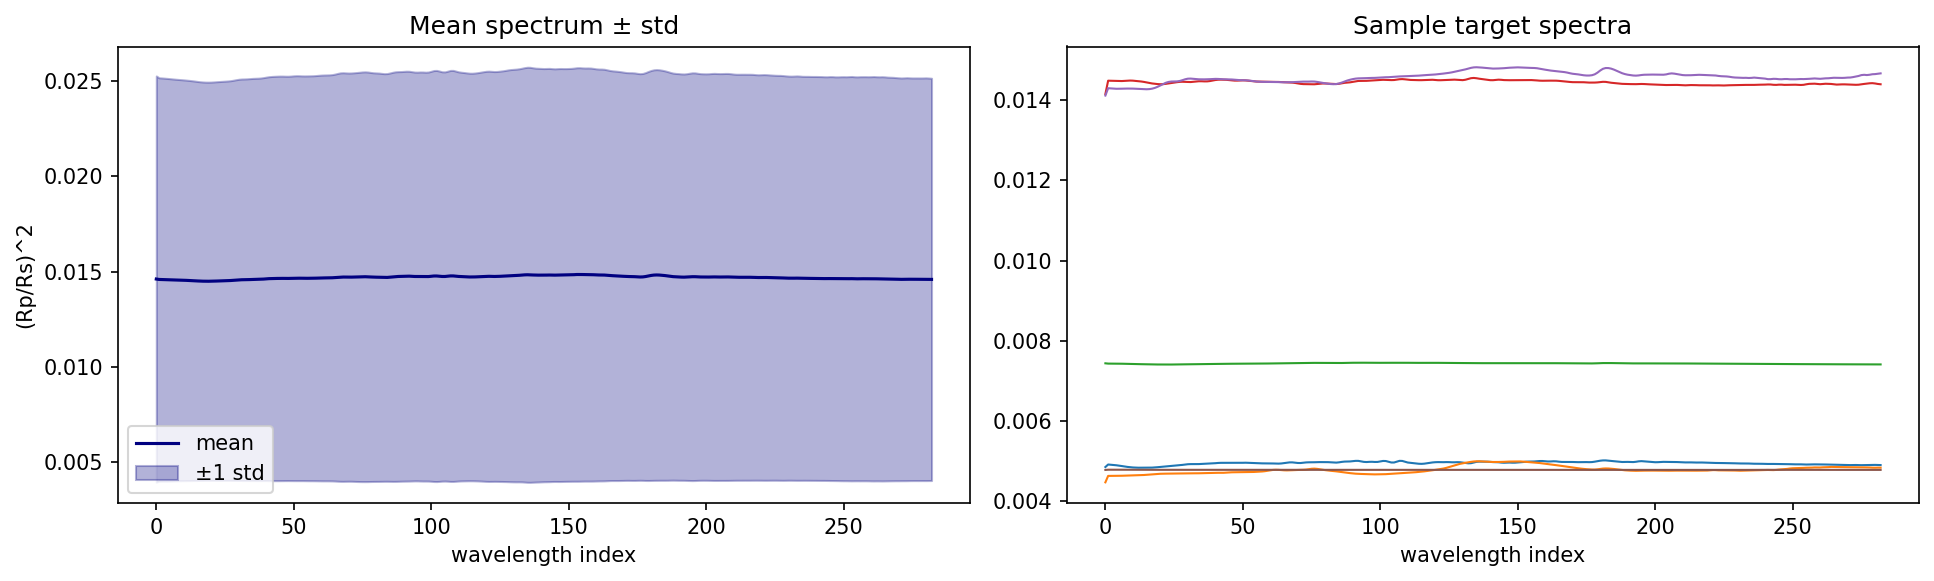
\includegraphics[width=0.85\linewidth]{figures/eda_target_spectra.png}
\caption{Left: dataset-wide mean spectrum $\pm$ 1$\sigma$. Right: a sample of individual planet spectra overlaid. The $y$-axis is $(R_p/R_s)^2$.}
\end{figure}

The left panel shows the mean spectrum (centred around $(R_p/R_s)^2 \approx 0.015$) with its $\pm 1\sigma$ envelope; the right panel overlays several individual spectra. Both reveal the same structure: \textbf{individual spectra are nearly flat in wavelength}, with the dominant variation being the \emph{overall depth level} (planet size), which differs substantially between planets. Within each planet, the spectral modulation is tiny relative to the depth offset.

\begin{figure}[H]
\centering
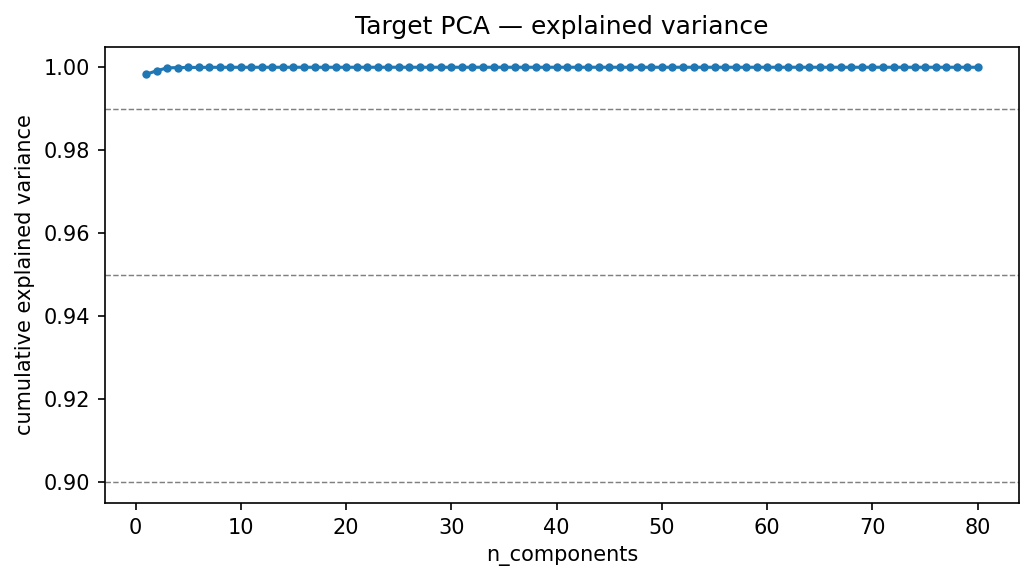
\includegraphics[width=0.85\linewidth]{figures/eda_pca_variance.png}
\caption{Cumulative explained variance of target PCA. The curve reaches $\approx$99.8\% at the first component and is essentially flat thereafter.}
\end{figure}

A PCA of the 283-dimensional target matrix confirms this quantitatively: \textbf{the first principal component alone captures $\approx$99.8\% of the variance}. The curve (shown from 0.90 to 1.00 on the $y$-axis across up to 80 components) is effectively a step function at component 1. The target is therefore \emph{nearly rank-1}: one number - the mean transit depth - explains almost everything, and the \textbf{atmospheric spectral features, the actual scientific signal, are a $\sim$0.2\% modulation} on top, buried in noise. This observation explains much of what follows: RMSE is nearly flat in the number of PCA components, and the score depends more on uncertainty quality than on spectral detail.

\subsection{Depth distribution and signal magnitude}

\begin{figure}[H]
\centering
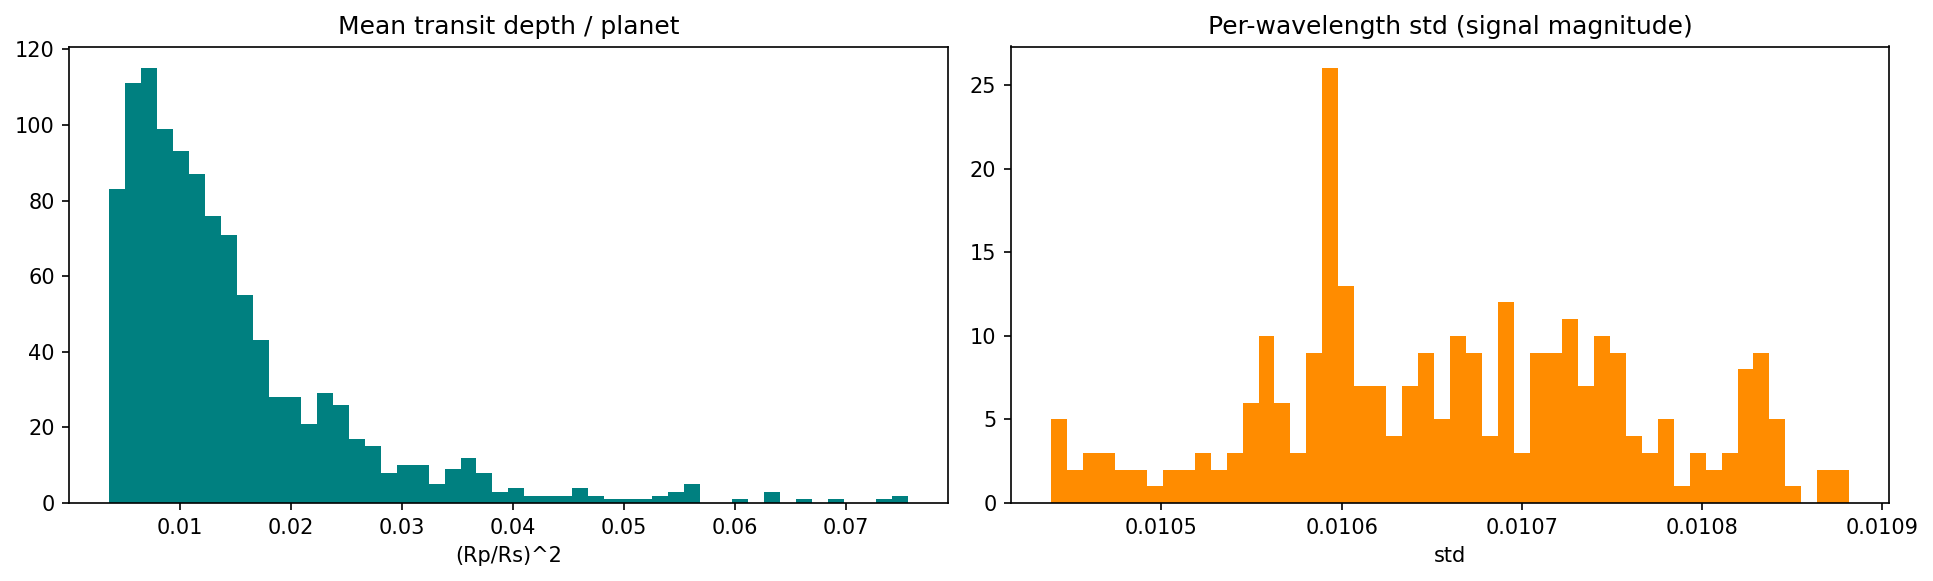
\includegraphics[width=0.85\linewidth]{figures/eda_depth_distribution.png}
\caption{Left: distribution of mean transit depth per planet. Right: per-wavelength standard deviation of the target across all planets.}
\end{figure}

The mean transit depth per planet is right-skewed, with most planets in the range 0.008--0.012 $(R_p/R_s)^2$ and a tail extending to $\sim$0.07, reflecting a wide range of planet-to-star size ratios. The right panel shows the per-wavelength standard deviation of targets across all planets: it is tightly concentrated around $\sim$0.0106 and nearly constant across wavelengths - direct evidence of the rank-1 structure, since most cross-planet variance is explained by the scalar depth level alone.

\subsection{Light curves and heteroscedastic channel noise}

\begin{figure}[H]
\centering
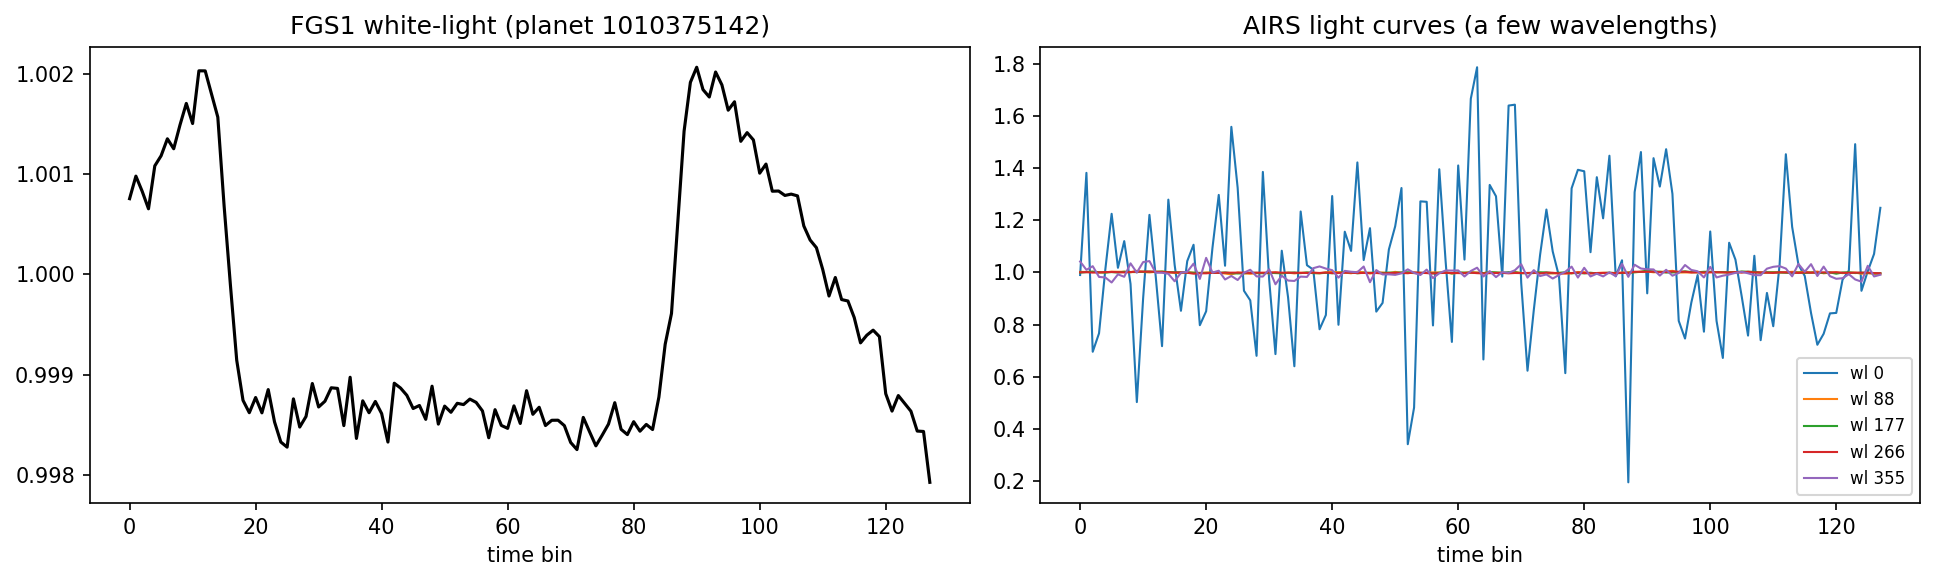
\includegraphics[width=0.85\linewidth]{figures/eda_light_curve.png}
\caption{Left: FGS1 white-light light curve (planet 1010375142) over 130 time bins, showing a clear transit dip. Right: AIRS per-wavelength curves for selected wavelength indices (0, 89, 177, 266, 355); wavelength 0 is notably noisier than the rest.}
\end{figure}

The FGS1 white-light curve (left) shows a \textbf{clean transit dip} spanning roughly time bins 20--100, validating the calibration and detrending pipeline. The AIRS per-wavelength curves (right) are significantly noisier: all channels fluctuate around a normalised flux of $\sim$1.0, but \textbf{the first AIRS channel (wavelength index 0) exhibits markedly higher noise} relative to the interior channels. This \textbf{heteroscedastic, wavelength-dependent noise structure} directly motivates per-wavelength uncertainty calibration rather than a single global $\sigma$.

\subsection{Stellar and orbital metadata}

\begin{figure}[H]
\centering
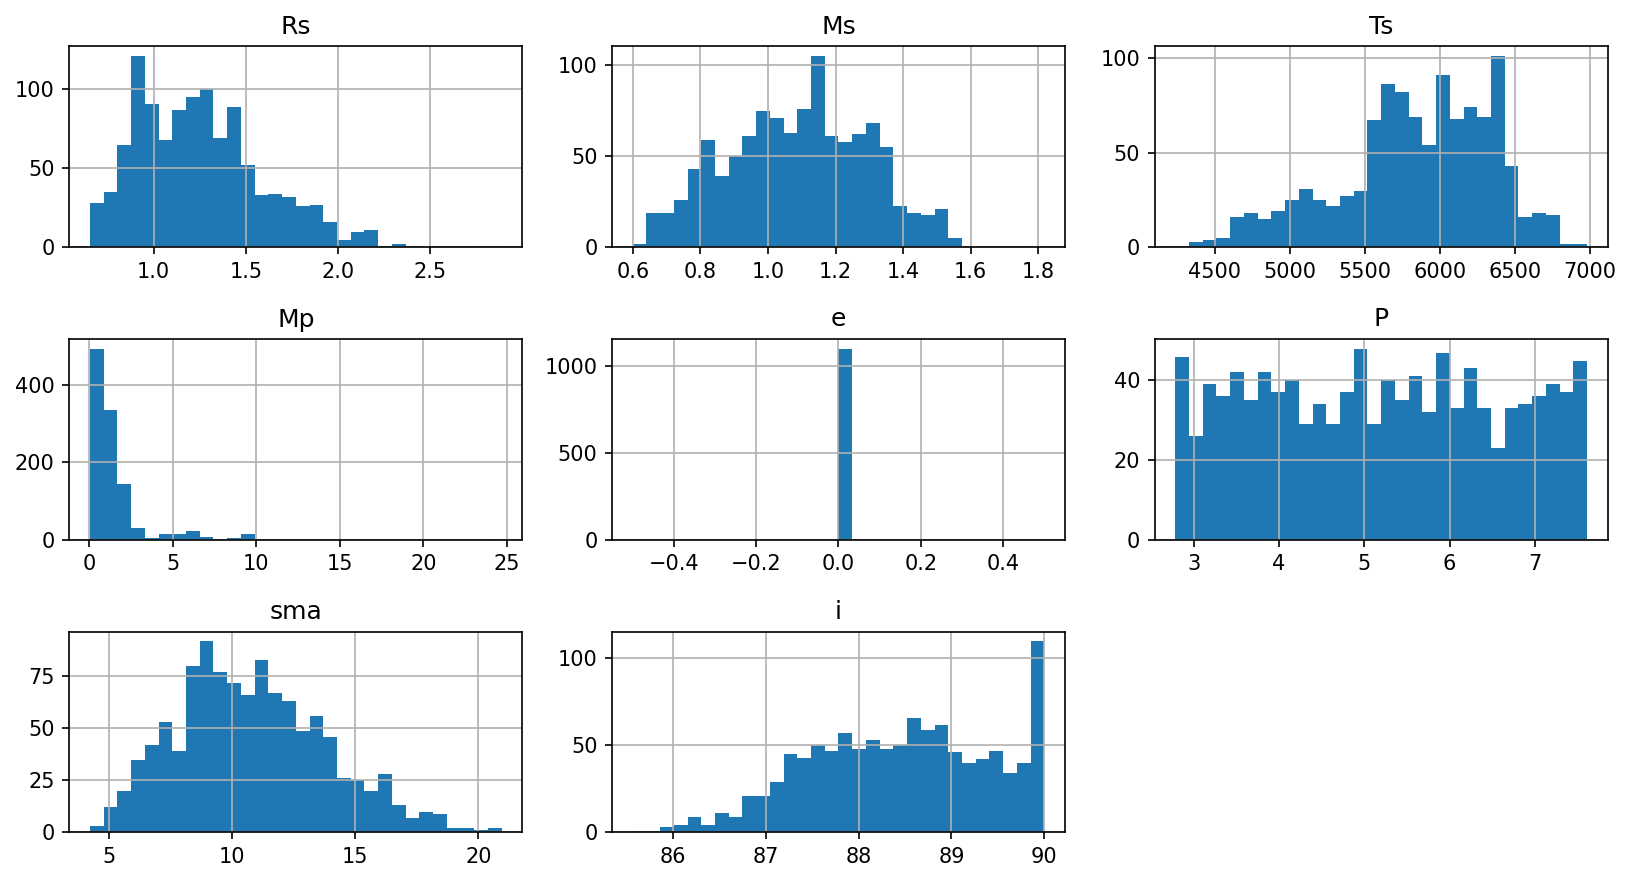
\includegraphics[width=0.85\linewidth]{figures/eda_star_metadata.png}
\caption{Distributions of stellar and orbital parameters across the training set (8 panels).}
\end{figure}

The metadata covers eight quantities: stellar radius $R_s$ and mass $M_s$ (both centred around 1.0--1.2 solar units), effective temperature $T_s$ (concentrated at 5500--6000 K), planet mass $M_p$ (heavily right-skewed, with most values near zero), orbital eccentricity (strongly peaked at 0, consistent with circularised close-in orbits), orbital period (3--7 days), semi-major axis, and inclination (tightly clustered near 90°, consistent with edge-on transiting geometry). These features are included as auxiliary predictors with log-transforms and depth interactions (\S{}5.2); their distributions are unimodal and well-behaved, posing no preprocessing challenge.

\textbf{EDA takeaway.} The problem is a \emph{needle-in-haystack}: an easy, dominant depth signal plus a tiny, hard, low-SNR spectral modulation. A good GLL score requires both a reasonable mean \textbf{and} an uncertainty matched to the wavelength-dependent noise - neither alone is sufficient.

\section{Methodology}

\subsection{Pipeline overview}

Each planet's raw detector data passes through the following stages before entering any model:

\begin{lstlisting}
Raw AIRS/FGS signals
  -> ADC correction (gain/offset)
  -> Correlated double sampling (CDS) + temporal binning
  -> Dead/hot pixel masking + dark subtraction + flat-field division
  -> NaN interpolation
  -> Light-curve extraction  (AIRS per-wavelength, FGS white-light)
  -> Transit boundary detection  (FGS-driven, derivative-based)
  -> Normalisation + polynomial detrending + smoothing
  -> Physics-based feature engineering
\end{lstlisting}

All stages are controlled by a unified configuration object. The same calibrated light curves feed both the tabular feature path and the deep-model tensor path, ensuring the two model classes share an identical preprocessing front-end.

\subsection{Physics-based feature engineering}

We extract approximately 100-150 features per planet, organised into five groups:

\begin{itemize}
\item \textbf{Transit depth.} Per-wavelength transit depth $d_\lambda = 1 - \bar{f}_{\text{in},\lambda}/\bar{f}_{\text{oot},\lambda}$, together with its mean, median, minimum, 5th/10th percentile, standard deviation, noise-weighted average, and mid-transit value. This is the most informative group, since $d_\lambda \approx (R_p/R_s)^2$.

\item \textbf{Multi-scale spectral.} The 283 per-wavelength depths are binned at multiple scales (bin sizes 1, 2, 4, 8, 16, 32, 64); within each bin we compute mean, median, standard deviation, linear slope, and second-order curvature. This exploits the known spectral smoothness of atmospheric transmission features.

\item \textbf{Transit shape.} Ingress and egress slopes, transit duration, mid-transit flux, in-transit symmetry, bottom curvature, out-of-transit left/right trends, and baseline drift - derived from both the FGS white-light curve and the wavelength-integrated AIRS curve.

\item \textbf{Noise and calibration proxies.} Out-of-transit standard deviation (mean and max), in-transit standard deviation, residual standard deviation after detrending, signal-to-noise ratio, CDS noise proxy, bad and hot pixel counts, flat-field variance, dark current level, and read noise level. These directly model the instrument noise budget and are the most important group in the feature-importance ranking.

\item \textbf{Stellar and orbital metadata.} Stellar radius $R_s$, mass $M_s$, effective temperature $T_s$, surface gravity $\log g$, and orbital period - each in raw and log-transformed form, plus depth-times-stellar-parameter interaction terms.
\end{itemize}

\subsection{Target PCA and per-component regression}

Rather than training 283 independent regressors, we reduce the output space via PCA on the target matrix and regress each principal component separately:

\[
Z = \mathrm{PCA}(Y),\quad \hat{z}_k = f_k(X),\quad \hat{Y} = \mathrm{PCA}^{-1}(\hat{Z}).
\]

This compresses 283 outputs to typically 20-40 components, enforces spectral smoothness via the PCA basis, and regularises against overfitting. Uncertainty in the original spectral space is obtained by propagating through the inverse PCA transform and combining with a per-wavelength residual RMSE:

\[
\hat{\sigma}^2_{Y,j} = \sum_k W_{kj}^2\,\hat{\sigma}^2_{Z,k} + \hat{\varepsilon}^2_j,
\]

where $W_{kj}$ are the PCA loading entries, $\hat{\sigma}^2_{Z,k}$ is the per-component predictive variance from the base regressor, and $\hat{\varepsilon}_j$ is estimated on a held-out calibration split.

\textbf{Efficient $n_{\text{components}}$ sweep.} PCA components are nested: the first $k$ components of a $K_{\max}$-component fit equal those of a stand-alone $k$-component fit. Combined with the independence of per-component regressors, this means we can fit \emph{once} at $K_{\max}$ and evaluate every smaller $k$ by truncating the component sum - bit-for-bit identical to running full cross-validation at each $k$, but without the cost factor of the grid.

\subsection{Model families}

All tabular estimators are wrapped in the Target-PCA layer and differ only in the base regressor for each PCA component. The 22 models benchmarked in \S{}6.1 span seven families:

\begin{center}\small
\begin{tabular}{@{}p{0.28\linewidth} p{0.64\linewidth}@{}}
\toprule
\textbf{Family} & \textbf{Models} \\
\midrule
Linear & Ridge, Lasso, ElasticNet \\
Bayesian / probabilistic & Bayesian Ridge, ARD, Gaussian Process, NGBoost \\
Kernel / SVM & SVR, Kernel Ridge \\
Neighbours & KNN \\
Tree ensembles & Random Forest, Extra Trees, Hist Gradient Boosting, LightGBM, XGBoost \\
Shallow neural & MLP \\
Deep sequence & CNN1D, TCN, LSTM, GRU, Transformer, Autoencoder+MLP \\
\bottomrule
\end{tabular}
\end{center}

Uncertainty is drawn from the most natural source per family: \textbf{Bayesian predictive standard deviation} for Bayesian Ridge, ARD, Gaussian Process, and NGBoost; \textbf{ensemble standard deviation across trees} for Random Forest and Extra Trees; and a \textbf{residual-RMSE fallback} for all point estimators (Ridge, Lasso, SVR, KNN, the gradient-boosting machines). The residual-RMSE fallback is a constant fitted on the calibration split - it is wide by construction and is the primary reason these models cluster at GLL = 0.

Two additional families - hybrid (Bayesian Ridge with a boosting residual correction) and mean-shift (explicit depth/shape decomposition) - are implemented but excluded from the main benchmark; the mean-shift ablation is discussed in \S{}6.4.

\subsection{PHC: Physics-conditioned Heteroscedastic Calibration}

The GLL grades $\sigma$ as strongly as $\mu$, motivating an explicit recalibration stage. PHC standardises each model's uncertainty in three steps, all fitted on a held-out calibration split (20\% of each training fold) to prevent a circular NLL.

\textbf{Step 1 - Per-wavelength scale (closed form).} An independent scale $s_j$ replaces a single global multiplier. Because the GLL decomposes additively over wavelengths and $s_j$ affects only column $j$, setting $\partial(\text{GLL})/\partial s_j = 0$ yields the closed-form optimum:

\[
\boxed{\;s_j^\star = \sqrt{\frac{1}{N}\sum_{i=1}^N \left(\frac{y_{ij}-\mu_{ij}}{\sigma_{ij}}\right)^2}\;}
\]

the root-mean-square of the normalised residuals in column $j$ - no iteration required.

\textbf{Step 2 - Feature-conditioned row multiplier.} After applying Step 1, the per-planet residual structure is modelled: the optimal per-row multiplier

\[
t_i = \sqrt{\frac{1}{M}\sum_{j=1}^M \left(\frac{r_{ij}}{s_j\,\sigma_{ij}}\right)^2}
\]

is predicted from the noise features via log-space ridge regression ($\log t_i \sim X_i$), so noisier observations receive proportionally wider intervals.

\textbf{Step 3 - GLL-weighted family mixture.} Model families can be combined as a Gaussian mixture, with weights $\propto \mathrm{softmax}(\text{validation GLL}/\tau)$, prioritising better-calibrated families.

PHC places every model's $\sigma$ on a common footing for the synchronised comparison in \S{}6.6. Its empirical effect on the score is examined critically in \S{}6.3.

\subsection{Deep sequence models}

Six architectures are trained end-to-end on calibrated light curves as comparative baselines. Input tensors have shape $[\text{planets} \times T \times C]$, where $T = 128$ time steps and $C = 65$ channels (1 FGS white-light curve concatenated with 64 wavelength-binned AIRS curves), standardised per channel.

All architectures share a dual-head output layer producing $(\mu, \log\hat{\sigma})$ per target and are trained with a Gaussian NLL loss, where $\sigma = \mathrm{softplus}(\log\hat{\sigma}) + \varepsilon$ ensures positivity:

\[
\mathcal{L} = \frac{1}{N}\sum_i \left[\frac{(y_i - \mu_i)^2}{2\sigma_i^2} + \log\sigma_i\right].
\]

\begin{itemize}
\item \textbf{CNN1D.} Three Conv1D layers with kernel sizes 7, 5, 3 and progressively widened feature maps, batch normalisation, ReLU, and adaptive average pooling.
\item \textbf{TCN (Temporal Convolutional Network).} Four dilated Conv1D layers with exponentially increasing dilation factors (1, 2, 4, 8), yielding a receptive field spanning the full light curve with few parameters.
\item \textbf{LSTM / GRU.} Two-layer recurrent networks; the final hidden state is projected to the output head.
\item \textbf{Transformer.} Linear input projection followed by a three-layer TransformerEncoder (4 attention heads, $4\times$ feedforward expansion, pre-layer normalisation), then global average pooling over time.
\item \textbf{Autoencoder+MLP.} A bottleneck encoder compresses the time series to a latent vector, from which an MLP predicts the spectrum.
\end{itemize}

An optional target PCA (30 components) mirrors the tabular setup, with uncertainty propagated through the inverse transform as in \S{}5.3. Training uses the Adam optimiser with early stopping (patience 20, maximum 200 epochs).

\subsection{Evaluation protocol}

\begin{itemize}
\item \textbf{Cross-validation.} GroupKFold by planet - no planet appears in both train and validation within any fold.
\item \textbf{Calibration holdout.} 20\% of each training fold is reserved to fit the per-wavelength residual RMSE and the PHC calibrator; the evaluation fold is never used for $\sigma$ fitting.
\item \textbf{Metric.} The official normalised GLL score, with the naive reference computed from the training-fold targets.
\item \textbf{Synchronised ML-vs-Deep comparison.} Both model classes are evaluated on the same held-out planets with the same PHC calibration and the same naive reference, eliminating all evaluation confounds.
\end{itemize}

\section{Experiments \& Results}

\textbf{How to read the result tables.} We report two complementary protocols.

\begin{itemize}
\item \textbf{Merged benchmark (\S{}6.1):} covers all 22 models, but mixes ML cross-validation results with deep single-split results; useful for orientation rather than for the final ML-vs-Deep claim.
\item \textbf{Synchronized comparison (\S{}6.6):} representative ML and deep models evaluated on the \emph{same} held-out planets with the \emph{same} PHC calibration and the \emph{same} naive reference - the only valid basis for an ML-vs-Deep claim.
\end{itemize}

In all result tables, \emph{cov 1$\sigma$} denotes empirical one-standard-deviation coverage: the fraction of target values satisfying $y_{ij}\in[\mu_{ij}-\sigma_{ij},\,\mu_{ij}+\sigma_{ij}]$. For a well-calibrated Gaussian model this should be near 68\%; much larger values indicate over-wide, under-confident uncertainties.

\subsection{Model-family benchmark (22 models)}

We cross-validate every tabular model on identical folds under the official metric. Deep model results come from a single held-out split and are included in the ranking table for orientation. The full ranking:

\begin{center}\scriptsize
\resizebox{\linewidth}{!}{%
\begin{tabular}{@{}l l l l l l l@{}}
\toprule
Family & Model & Ariel GLL & RMSE & NLL & cov 1$\sigma$ & $\bar{\sigma}$ \\
\midrule
deep & cnn1d & 0.227 & 0.00312 & -5.76 & 0.76 & 0.0023 \\
deep & transformer & 0.226 & 0.00207 & -5.75 & 0.72 & 0.0020 \\
trees & extra\_trees & 0.215 & 0.00253 & -5.65 & 0.94 & 0.0031 \\
trees & random\_forest & 0.199 & 0.00273 & -5.52 & 0.93 & 0.0036 \\
bayesian & ngboost & 0.167 & 0.00221 & -5.29 & 0.95 & 0.0047 \\
deep & tcn & 0.167 & 0.00373 & -5.32 & 0.71 & 0.0033 \\
bayesian & ard & 0.143 & 0.00247 & -5.11 & 0.94 & 0.0054 \\
deep & gru & 0.129 & 0.00448 & -5.03 & 0.84 & 0.0040 \\
bayesian & bayesian\_ridge & 0.093 & 0.00352 & -4.73 & 0.95 & 0.0078 \\
deep & lstm & 0.000 & 0.01030 & -4.08 & 0.82 & 0.0103 \\
trees & hist\_gradient\_boosting & \textbf{0.000} & 0.00264 & -1.28 & 1.00 & 0.280 \\
trees & xgboost & \textbf{0.000} & \textbf{0.00237} & -1.30 & 1.00 & 0.279 \\
trees & lightgbm & \textbf{0.000} & 0.00261 & -1.29 & 1.00 & 0.278 \\
kernel\_svm & svr & 0.000 & 0.00439 & -0.73 & 1.00 & 0.485 \\
kernel\_svm & kernel\_ridge & 0.000 & 0.00517 & -0.53 & 1.00 & 0.595 \\
neighbors & knn & 0.000 & 0.00541 & -0.53 & 1.00 & 0.595 \\
linear & lasso & 0.000 & 0.00252 & -1.24 & 1.00 & 0.298 \\
linear & elastic\_net & 0.000 & 0.00280 & -1.15 & 1.00 & 0.325 \\
linear & ridge & 0.000 & 0.00643 & -0.35 & 1.00 & 0.708 \\
neural & mlp & 0.000 & 0.00635 & -0.37 & 1.00 & 0.703 \\
bayesian & gaussian\_process & 0.000 & 0.01066 & -3.91 & 0.92 & 0.016 \\
deep & autoencoder\_mlp & 0.000 & 0.01059 & -3.87 & 0.87 & 0.0129 \\
\bottomrule
\end{tabular}
}
\end{center}

\begin{figure}[H]
\centering
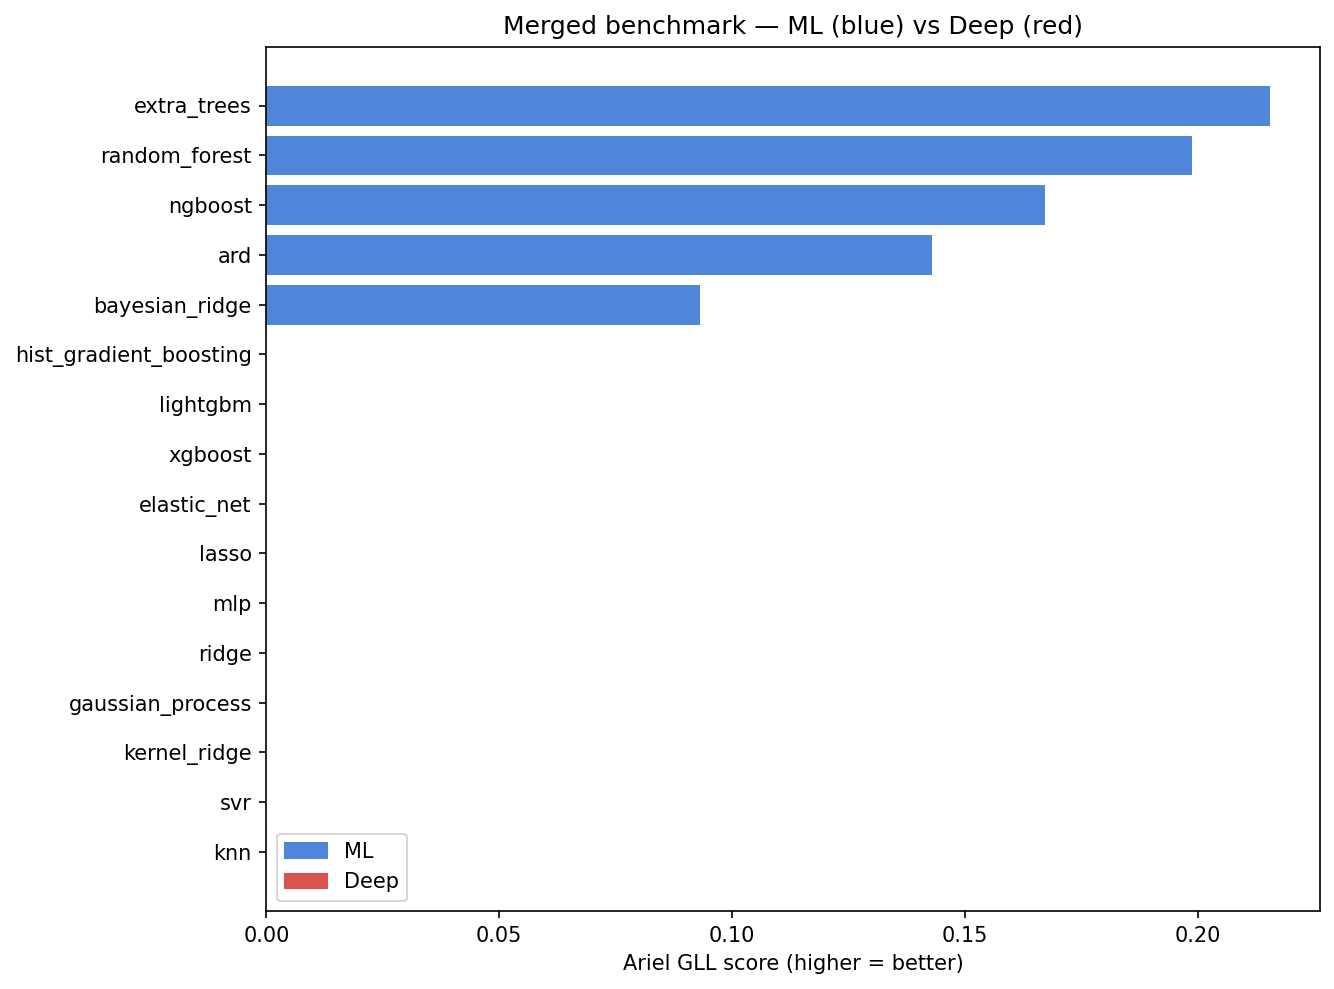
\includegraphics[width=0.85\linewidth]{figures/merged_benchmark.png}
\caption{Ariel GLL scores for the 16 tabular ML models ranked by cross-validation performance (blue). Only ML models are shown; deep model results are evaluated separately and reported in \S{}6.6.}
\end{figure}

The results split into two clear clusters. Models with \textbf{informative uncertainty} - the tree ensembles (Extra Trees \cite{geurts2006}, Random Forest \cite{breiman2001}) and the Bayesian models (NGBoost \cite{duan2020}, ARD, Bayesian Ridge) - achieve GLL $>$ 0. All remaining 16 models score GLL = 0. This cluster has two distinct failure modes: (i) \textbf{point estimators} (Ridge, Lasso, ElasticNet, MLP, SVR, Kernel Ridge, KNN, and the gradient-boosting machines) whose residual-RMSE-fallback uncertainty is far too wide ($\bar{\sigma}\approx 0.28$-$0.71$, coverage 1.0) - with XGBoost \cite{chen2016} being the most striking case: \textbf{best RMSE (0.00237) yet GLL = 0}; and (ii) two weak deep models (LSTM, Autoencoder+MLP) whose $\bar{\sigma}$ is reasonable ($\approx 0.01$-$0.013$) but whose mean is poor (RMSE $\approx 0.010$, roughly $4\times$ the best). Both failure modes confirm that a good score requires \emph{both} an accurate mean \emph{and} a well-scaled uncertainty.

\textit{Note on protocol mixing.} Deep results come from a single held-out split without PHC; ML results come from 3-fold cross-validation with PHC. This table is for screening only - \S{}6.6 corrects the comparison under an identical protocol.

\subsection{Target-PCA component sweep}

Sweeping $n_{\text{components}}\in\{10,\dots,50\}$ leaves RMSE essentially unchanged ($\approx 0.0061$ for linear models), confirming the rank-1 EDA finding: extra components mostly capture noise. The efficient nested-sweep described in \S{}5.3 evaluates all values of $k$ from a single fit at $K_{\max}$, verified bit-for-bit against full cross-validation.

\subsection{PHC calibration ablation}

We vary only the uncertainty-calibration stage of Bayesian Ridge, keeping the mean predictor identical:

\begin{center}\small
\begin{tabular}{@{}p{0.32\linewidth} p{0.20\linewidth} p{0.20\linewidth}@{}}
\toprule
Calibration & Ariel GLL & NLL \\
\midrule
\textbf{none} (raw $\sigma$) & \textbf{0.127} & -4.99 \\
scalar (global) & 0.093 & -4.73 \\
per-wavelength (PHC Step 1) & 0.093 & -4.73 \\
feature-conditioned (PHC Step 2) & 0.063 & -4.45 \\
\bottomrule
\end{tabular}
\end{center}

\begin{figure}[H]
\centering
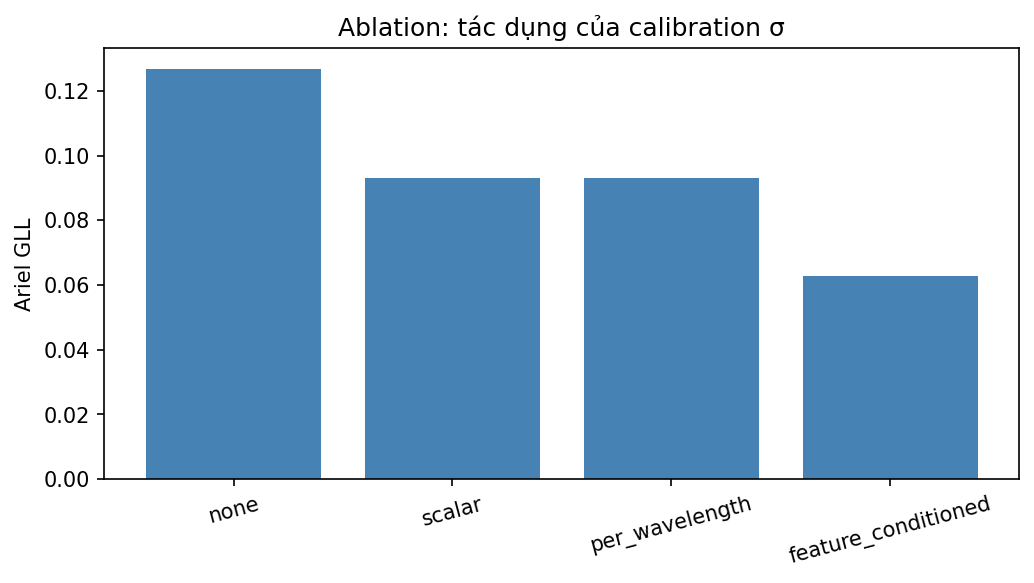
\includegraphics[width=0.85\linewidth]{figures/analysis_calibration_ablation.png}
\caption{Ariel GLL for Bayesian Ridge under four calibration regimes. GLL decreases monotonically with calibration complexity: no calibration (0.127), global scalar and per-wavelength calibration (both 0.093), and feature-conditioned calibration (0.063).}
\end{figure}

This is a \textbf{negative result, reported honestly}: the uncalibrated model scores highest; scalar and per-wavelength calibration identically reduce the score; feature-conditioning reduces it further by overfitting. The reliability diagram explains the mechanism:

\begin{figure}[H]
\centering
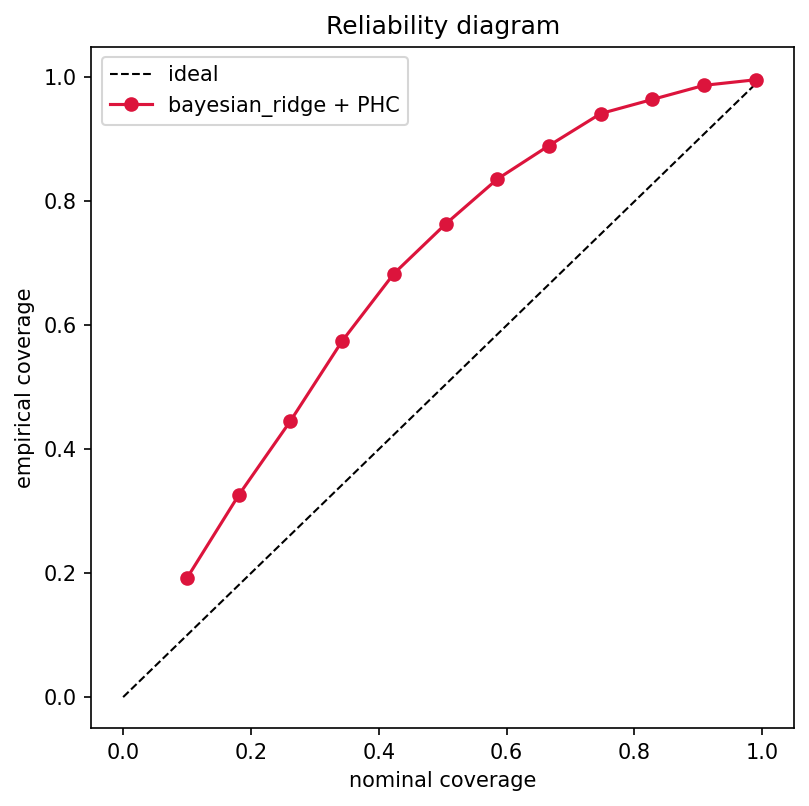
\includegraphics[width=0.85\linewidth]{figures/analysis_reliability.png}
\caption{Reliability diagram for Bayesian Ridge + PHC. The red curve lies above the ideal diagonal at all nominal coverage levels, indicating systematic under-confidence: predicted intervals are too wide throughout.}
\end{figure}

The empirical coverage curve lies consistently above the diagonal at all nominal levels, meaning the model's $\sigma$ is already too wide \emph{before} any recalibration. Two mechanisms explain this: (i) the base regressor already incorporates a per-wavelength residual RMSE into $\sigma$, making an additional per-wavelength scale redundant - which is why scalar and per-wavelength calibration score identically; and (ii) since the intrinsic $\sigma$ is already over-wide, any multiplicative adjustment widens it further, lowering GLL. \textbf{Conclusion:} on this dataset the models' intrinsic uncertainty is already adequate. PHC is theoretically grounded and valuable for standardising $\sigma$ across model families for the fair comparison in \S{}6.6, but it is not a score-improving step here.

\subsection{Mean-depth and shape decomposition (negative ablation)}

Motivated by the rank-1 EDA, we trained a decomposed model: predict the per-planet mean depth and the residual spectral shape separately, then recombine. Across many configurations this gave \textbf{no improvement} (linear models: +0.001-0.009 GLL; tree ensembles: worse by 0.03-0.04 GLL). Target-PCA already separates the rank-1 structure implicitly - the first principal component captures the depth level - making an explicit split redundant for linear models and harmful for trees. This approach is excluded from the main benchmark.

\subsection{Learning curve}

\begin{center}\small
\begin{tabular}{@{}p{0.22\linewidth} p{0.22\linewidth} p{0.22\linewidth}@{}}
\toprule
\#planets & Ariel GLL & RMSE \\
\midrule
50 & 0.009 & 0.00365 \\
100 & 0.000 & 0.00603 \\
200 & 0.000 & 0.00551 \\
400 & 0.000 & 0.00508 \\
800 & \textbf{0.105} & 0.00371 \\
1100 & 0.093 & 0.00352 \\
\bottomrule
\end{tabular}
\end{center}

\begin{figure}[H]
\centering
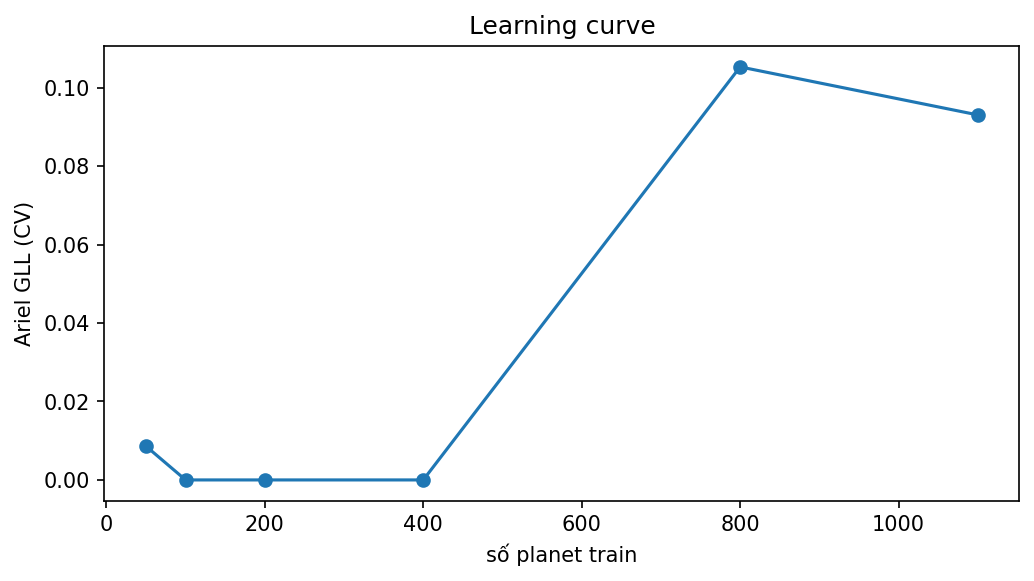
\includegraphics[width=0.85\linewidth]{figures/analysis_learning_curve.png}
\caption{Ariel GLL (cross-validation) versus number of training planets for Bayesian Ridge. GLL remains near zero for fewer than $\sim$800 planets, then rises sharply to $\sim$0.10 - a threshold effect characteristic of this low-signal retrieval task.}
\end{figure}

Bayesian Ridge cannot beat the naive baseline (GLL $\approx$ 0) until it sees approximately 800 planets, after which GLL rises to $\sim$0.10. RMSE decreases steadily with data volume. This threshold behaviour explains why early experiments at small training limits produced GLL $\approx$ 0 for most models, and it justifies using the full dataset for final evaluation.

\subsection{Synchronized ML vs Deep (headline result)}

To compare fairly, representative ML and deep models are evaluated on the \textbf{same held-out planets} with the \textbf{same per-wavelength PHC calibration} (fit on one half of a held-out split, applied to the other - leak-free) and the \textbf{same naive reference}:

\begin{center}\small
\begin{tabular}{@{}l l l l l@{}}
\toprule
Model & Type & Ariel GLL & RMSE & cov 1$\sigma$ \\
\midrule
\textbf{extra\_trees} & ml + PHC & \textbf{0.287} & 0.00250 & 0.77 \\
\textbf{random\_forest} & ml + PHC & \textbf{0.273} & 0.00258 & 0.82 \\
cnn1d & deep + PHC & 0.221 & 0.00349 & 0.74 \\
transformer & deep + PHC & 0.220 & 0.00226 & 0.68 \\
tcn & deep + PHC & 0.167 & 0.00400 & 0.74 \\
gru & deep + PHC & 0.119 & 0.00479 & 0.81 \\
bayesian\_ridge & ml + PHC & 0.074 & 0.00355 & 0.67 \\
lstm & deep + PHC & 0.000 & 0.01035 & 0.83 \\
autoencoder\_mlp & deep + PHC & 0.000 & 0.01064 & 0.84 \\
\bottomrule
\end{tabular}
\end{center}

\begin{figure}[H]
\centering
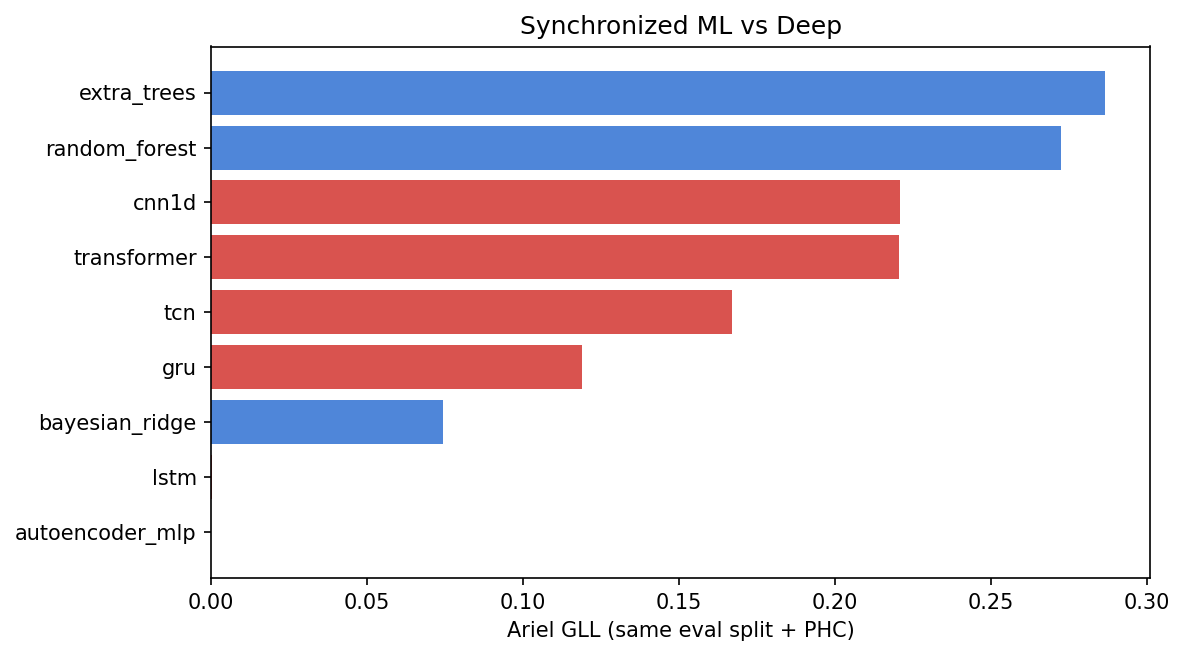
\includegraphics[width=0.85\linewidth]{figures/sync_ml_vs_deep.png}
\caption{Synchronized ML vs Deep comparison on identical held-out planets with identical PHC calibration. Blue bars: ML models; red bars: deep sequence models. Extra Trees (0.287) and Random Forest (0.273) lead; CNN1D and Transformer are competitive at $\sim$0.22.}
\end{figure}

\textbf{Under a fair protocol, tree ensembles clearly win} (Extra Trees 0.287, Random Forest 0.273), with deep CNN1D and Transformer competitive but behind ($\sim$0.22). This \textbf{reverses the apparent ranking} in the merged table (\S{}6.1), where CNN1D (0.227) appeared to beat Extra Trees (0.215). That apparent "deep wins" was a protocol artifact: deep numbers came from a single split without PHC while ML numbers came from cross-validation with PHC. The lesson is methodological - \emph{only a synchronized protocol yields a valid ML-vs-Deep comparison.}

\subsection{Feature importance}

\begin{figure}[H]
\centering
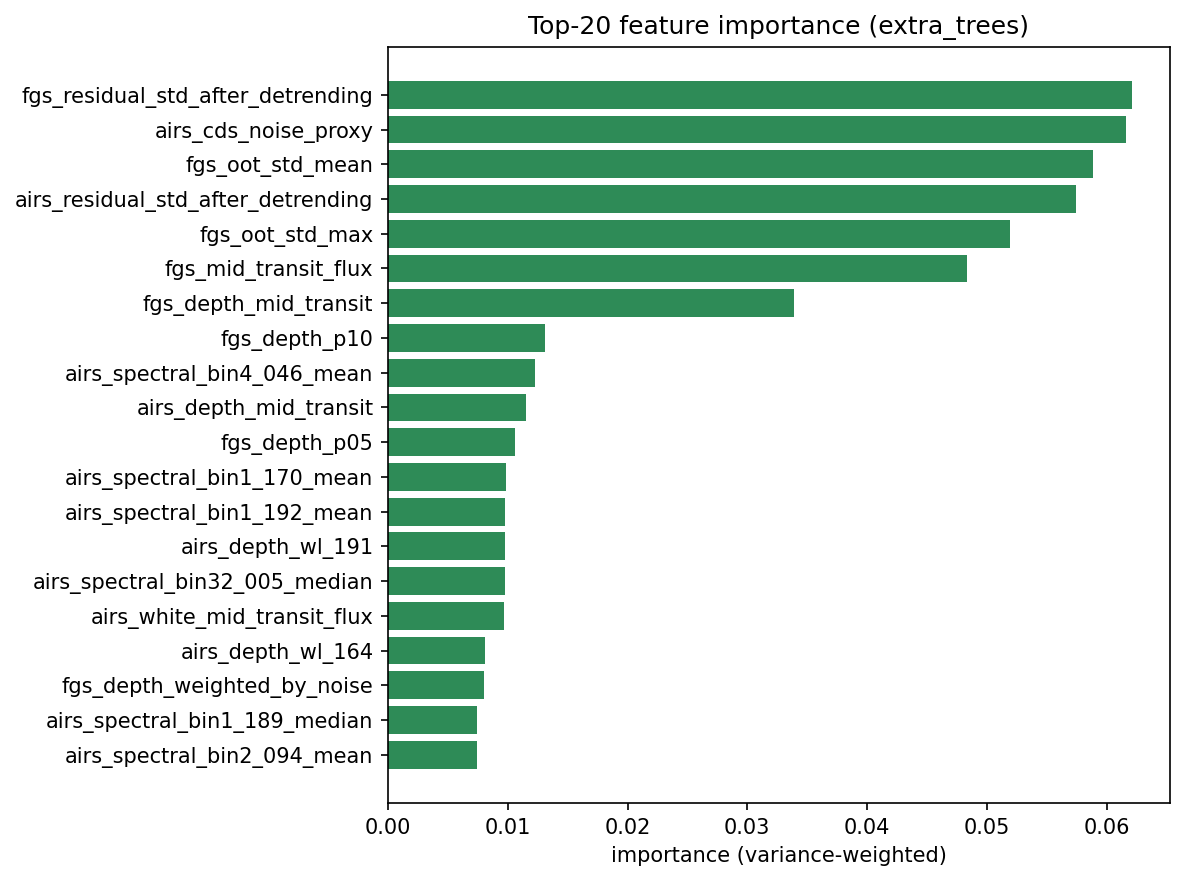
\includegraphics[width=0.85\linewidth]{figures/analysis_feature_importance.png}
\caption{Top-20 feature importances (variance-weighted) for Extra Trees \cite{geurts2006}. The four dominant features are all noise proxies: FGS residual std after detrending, AIRS CDS noise proxy, FGS out-of-transit std mean, and AIRS residual std after detrending.}
\end{figure}

The top-20 features split into two tiers. The first seven (importance $\geq 0.034$) are entirely noise and transit-shape proxies from FGS and AIRS: residual standard deviation after detrending, CDS noise proxy, out-of-transit standard deviation (mean and max), mid-transit flux, and mid-transit depth. The remaining 13 (importance $\approx 0.01$) are per-wavelength depths and multi-scale spectral bin features. This confirms that \textbf{noise-characterisation features dominate} - the model cares more about how reliable the signal is than about its fine spectral shape.

\subsection{Error analysis}

\begin{figure}[H]
\centering
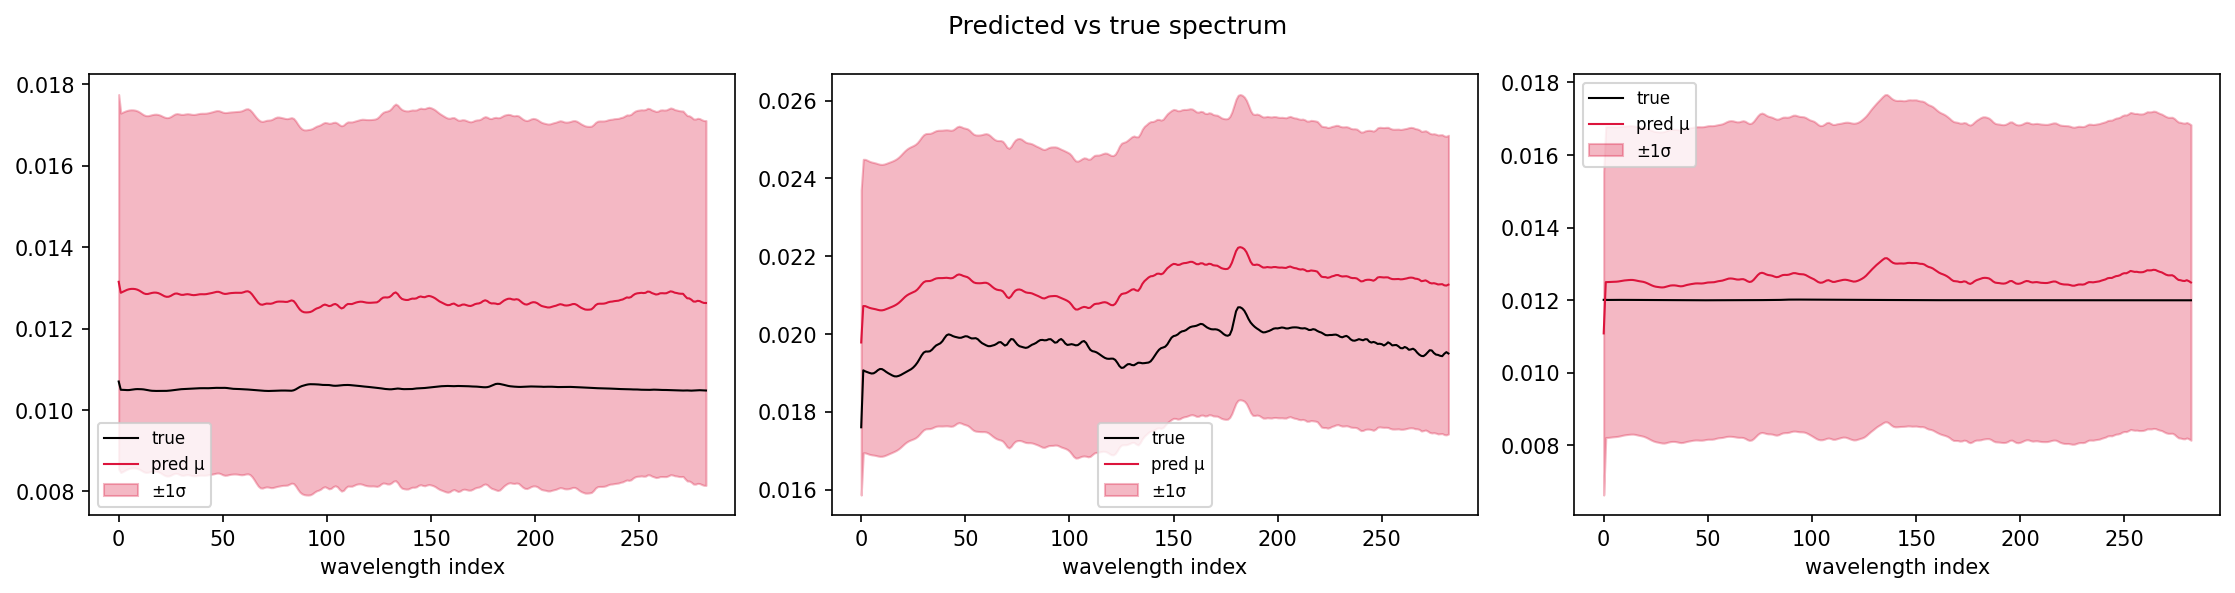
\includegraphics[width=0.85\linewidth]{figures/analysis_pred_vs_true.png}
\caption{Predicted vs true spectrum for three representative planets (Extra Trees). Black line: ground truth; red line: predicted mean $\mu$; pink band: $\pm 1\sigma$. The model captures the depth level well; the uncertainty band is substantially wider than the true spectral modulation.}
\end{figure}
\begin{figure}[H]
\centering
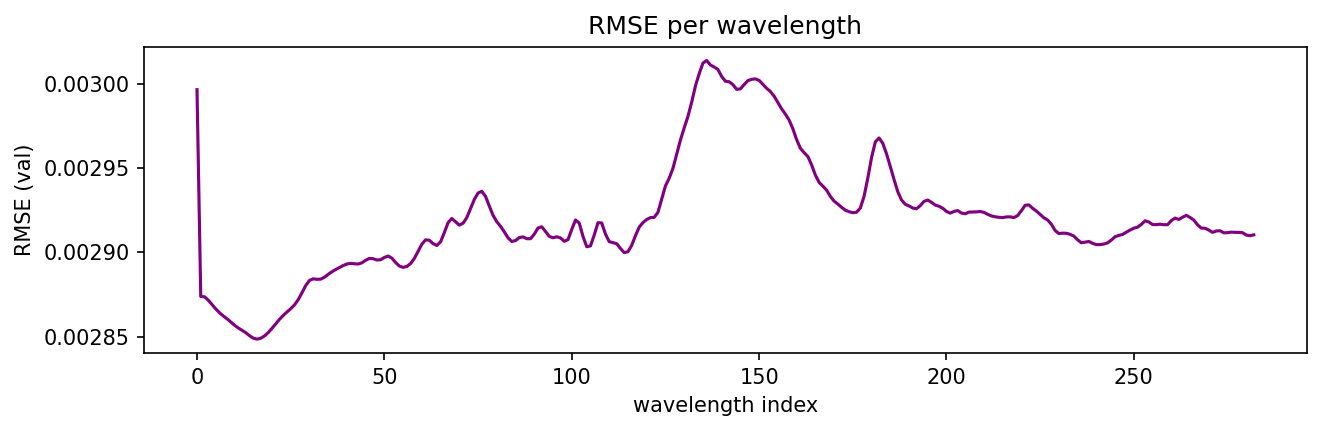
\includegraphics[width=0.85\linewidth]{figures/analysis_rmse_per_wavelength.png}
\caption{Per-wavelength RMSE for Extra Trees (cross-validation). Error is nearly uniform across all 283 channels ($\approx 0.00285$-$0.00315$), with a small spike at wavelength index 0 (the noisiest AIRS channel) and broader peaks around indices 130-150.}
\end{figure}

The per-wavelength RMSE lies in the narrow range $\approx 2.85\times10^{-3}$-$3.15\times10^{-3}$ across all 283 channels. The spike at wavelength index 0 matches the EDA finding that the first AIRS channel is noisier than the rest. The near-uniform profile is consistent with the rank-1 structure: once the depth level is predicted correctly, the residual low-SNR spectral modulation is equally difficult to recover at every wavelength.

\subsection{Statistical reliability}

\begin{center}\small
\begin{tabular}{@{}p{0.25\linewidth} p{0.35\linewidth} p{0.30\linewidth}@{}}
\toprule
Model & GLL (mean $\pm$ std) & RMSE (mean $\pm$ std) \\
\midrule
extra\_trees & 0.215 $\pm$ 0.025 & 0.00253 $\pm$ 0.00021 \\
bayesian\_ridge & 0.093 $\pm$ 0.026 & 0.00352 $\pm$ 0.00036 \\
ridge & 0.000 $\pm$ 0.000 & 0.00643 $\pm$ 0.00054 \\
\bottomrule
\end{tabular}
\end{center}

The fold-to-fold standard deviation ($\approx 0.025$) is much smaller than the gap between Extra Trees and Bayesian Ridge ($\approx 0.12$), so the ranking is \textbf{statistically robust} rather than a sampling artifact.

\subsection{Training cost and practical trade-offs}

Runtime differs substantially across families. Linear models train in seconds to minutes but score GLL = 0 due to uninformative uncertainty. Tree ensembles are more expensive but deliver the best calibrated uncertainty: Extra Trees requires roughly 40 minutes of wall-clock time while Random Forest takes roughly 6 hours in the recorded runs, yet both provide the best synchronized GLL. NGBoost is similarly expensive ($\sim$7 hours) while scoring below the tree ensembles. Gradient-boosting machines (XGBoost \cite{chen2016}, LightGBM \cite{ke2017}) train in minutes and achieve the best point-prediction RMSE but score GLL = 0. The practical recommendation is to use fast linear models for pipeline debugging, then allocate compute to Extra Trees for final scoring.


\section{Discussion \& Findings}

\begin{enumerate}
\item \textbf{Tree ensembles are the best models} on the official metric when compared fairly (Extra Trees 0.287, Random Forest 0.273); deep CNN1D and Transformer are competitive ($\sim$0.22); Bayesian linear is mid-pack ($\sim$0.09). The earlier "deep wins" impression was a protocol artifact - a direct lesson in experimental rigour.
\item \textbf{Uncertainty quality gates the GLL.} The score divides models into those with informative $\sigma$ (GLL $>$ 0) and point estimators (GLL = 0). XGBoost achieves the best RMSE yet scores 0 - emphatic evidence that \emph{a good mean is not enough}; the uncertainty must be informative and well-scaled.
\item \textbf{PHC is an honest negative result.} The closed-form per-wavelength calibration is theoretically optimal, but on this dataset the models' intrinsic $\sigma$ is already adequate - indeed over-wide - so recalibration is marginal to harmful and the feature-conditioned variant overfits. PHC remains valuable for standardising $\sigma$ across model families (enabling the fair comparison in \S{}6.6), but it is \textbf{not the dominant lever}.
\item \textbf{Strong data dependence.} GLL $\approx$ 0 below $\sim$800 planets, then a sharp rise - the small-data regime is a fundamental constraint, not a modelling failure.
\item \textbf{Physics noise-features matter most.} Tree importances are dominated by residual std, out-of-transit std, CDS noise proxy, and FGS-shape features, validating the physics-based feature engineering (\S{}5.2) over raw transit depth alone.
\item \textbf{Methodology over models.} The most transferable takeaway is that \textbf{protocol synchronisation} - identical evaluation split, identical calibration, identical naive reference - is required before any ML-vs-Deep claim is valid.
\end{enumerate}

\textbf{Synthesis.} GLL is governed by (a) having a model with good intrinsic uncertainty and (b) having enough data - more than by any explicit recalibration layer. The winning recipe is tree ensembles $+$ sufficient training planets $+$ physics-based noise features.


\section{Limitations \& Future Work}

\begin{itemize}
\item \textbf{Point-estimator uncertainty.} Linear, kernel, and gradient-boosting models score 0 only because they lack a usable $\sigma$. Conformal prediction \cite{angelopoulos2023} would provide distribution-free, data-adaptive intervals and likely lift these models substantially - the highest-value next step.
\item \textbf{More data and augmentation.} Given the learning-curve threshold at $\sim$800 planets, more training planets or physically motivated augmentation would benefit all models.
\item \textbf{Deep models under full cross-validation.} Deep results in the synchronized comparison are based on one held-out split; evaluating all deep architectures under full K-fold cross-validation would tighten the uncertainty around the comparison.
\item \textbf{Threats to validity.} The synchronized comparison is more fair than the merged benchmark, but it remains a single held-out evaluation rather than repeated nested cross-validation. Rankings may shift with a different split, more extensive hyperparameter tuning, or a larger synthetic training set. Compute constraints also meant that deep architectures and expensive probabilistic models were not tuned as exhaustively as the tabular tree ensembles.
\item \textbf{Tree and deep ensembling.} The GLL-weighted mixture (PHC Step 3) could combine the complementary strengths of tree ensembles and CNN, potentially exceeding either individually.
\item \textbf{Improved spectral decomposition.} A learned decomposition that handles the mean depth and residual spectral shape separately - rather than the simple mean-subtraction approach we tested - may still offer gains; our current version did not.
\end{itemize}


\section{Conclusion}

We presented a complete, tested pipeline for probabilistic atmospheric-spectrum retrieval from the Ariel Data Challenge 2025 \cite{mugnai2025} and a systematic, metric-faithful comparison of 22 models across seven families, including deep sequence baselines. Through a protocol-synchronized evaluation we established that tree ensembles win on the official GLL metric, that uncertainty quality - not point-prediction accuracy - determines success, and that the proposed PHC calibration, while theoretically grounded, offers only marginal empirical gains because intrinsic model uncertainty is already adequate. We documented a sharp learning-curve threshold at $\sim$800 training planets and confirmed that physics-based noise features dominate the feature importances. All results, including negative ones, are reported in full. The core methodological lesson is that fair ML-vs-Deep comparisons require strict protocol synchronisation: identical evaluation split, identical calibration, and identical naive reference.


\section{Contributions \& Reproducibility}

\subsection{Member contributions}

\begin{center}\small
\begin{tabular}{@{}p{0.32\linewidth} p{0.58\linewidth}@{}}
\toprule
Member & Main responsibilities \\
\midrule
\_[Member 1]\_ & Preprocessing and calibration pipeline; feature engineering \\
\_[Member 2]\_ & Model families, Target-PCA, benchmark harness \\
\_[Member 3]\_ & PHC and uncertainty calibration; metric; analysis and figures \\
\_[Member 4]\_ & Deep sequence models; synchronized comparison; report writing \\
\bottomrule
\end{tabular}
\end{center}

\subsection{Reproducibility}

\begin{itemize}
\item \textbf{Code.} The codebase is structured as flat Python modules \cite{pedregosa2011} covering preprocessing, feature engineering, models, metrics, training, estimators, deep models, and configuration - importable directly without package installation.
\item \textbf{Notebooks.} Four Kaggle notebooks cover the full pipeline: feature preparation, tabular model training with PHC calibration and submission generation, sequence tensor preparation, and deep-model training with the synchronized comparison. Separate analysis notebooks reproduce every table and figure in this report.
\item \textbf{Determinism.} Fixed random seeds, GroupKFold by planet identifier, and a 20\% sigma-calibration holdout are used throughout, ensuring reproducibility across runs.
\item \textbf{Unit tests.} A pytest test suite on synthetic data covers models, metric, training loops, calibration, sequence construction, and the efficient $n_{\text{components}}$ sweep.
\end{itemize}


\begin{thebibliography}{10}

\bibitem{mugnai2025}
Mugnai, L.~V., et al.\ (2025).
\newblock Ariel Machine Learning Data Challenge 2025: overview and results.
\newblock \textit{arXiv}:2505.08940.

\bibitem{tinetti2018}
Tinetti, G., et al.\ (2018).
\newblock A chemical survey of exoplanets with ARIEL.
\newblock \textit{Experimental Astronomy}, 46(1-2), 135-209.

\bibitem{pedregosa2011}
Pedregosa, F., et al.\ (2011).
\newblock Scikit-learn: Machine Learning in Python.
\newblock \textit{Journal of Machine Learning Research}, 12, 2825-2830.

\bibitem{geurts2006}
Geurts, P., Ernst, D., and Wehenkel, L.\ (2006).
\newblock Extremely randomized trees.
\newblock \textit{Machine Learning}, 63(1), 3-42.

\bibitem{breiman2001}
Breiman, L.\ (2001).
\newblock Random Forests.
\newblock \textit{Machine Learning}, 45(1), 5-32.

\bibitem{duan2020}
Duan, T., et al.\ (2020).
\newblock NGBoost: Natural Gradient Boosting for Probabilistic Prediction.
\newblock In \textit{Proc.\ 37th International Conference on Machine Learning (ICML)}, 2817-2826.

\bibitem{chen2016}
Chen, T., and Guestrin, C.\ (2016).
\newblock XGBoost: A Scalable Tree Boosting System.
\newblock In \textit{Proc.\ 22nd ACM SIGKDD Conference on Knowledge Discovery and Data Mining}, 785-794.

\bibitem{ke2017}
Ke, G., et al.\ (2017).
\newblock LightGBM: A Highly Efficient Gradient Boosting Decision Tree.
\newblock In \textit{Advances in Neural Information Processing Systems (NeurIPS)}, 30.

\bibitem{vaswani2017}
Vaswani, A., et al.\ (2017).
\newblock Attention Is All You Need.
\newblock In \textit{Advances in Neural Information Processing Systems (NeurIPS)}, 30, 5998-6008.

\bibitem{angelopoulos2023}
Angelopoulos, A.~N., and Bates, S.\ (2023).
\newblock A Gentle Introduction to Conformal Prediction and Distribution-Free Uncertainty Quantification.
\newblock \textit{Foundations and Trends in Machine Learning}, 16(4), 494-591.

\end{thebibliography}


\section{Appendix}

\subsection{Full benchmark results}

The complete 22-model ranking with all metric columns is reproduced in the table in \S{}6.1.

\subsection{PHC closed-form derivation}

For column $j$ with scale $s_j$, the per-column log-likelihood is
\[
\mathcal{L}_j = \sum_{i=1}^N \left[-\log(s_j\sigma_{ij}) - \frac{1}{2}\left(\frac{r_{ij}}{s_j\sigma_{ij}}\right)^2\right] + \text{const}.
\]
Setting $\partial\mathcal{L}_j/\partial s_j = 0$:
\[
-\frac{N}{s_j} + s_j^{-3}\sum_{i=1}^N\left(\frac{r_{ij}}{\sigma_{ij}}\right)^2 = 0 \quad\Longrightarrow\quad s_j^{\star\,2} = \frac{1}{N}\sum_{i=1}^N \left(\frac{r_{ij}}{\sigma_{ij}}\right)^2.
\]
The per-row multiplier in Step 2 is derived identically, summing over wavelengths instead of planets.

\subsection{Key hyperparameters}

\begin{itemize}
\item Target PCA: $n_{\text{components}} = 24$ (benchmark) / 30 (deep and synchronized); GroupKFold with 3-5 folds; calibration holdout fraction 0.2.
\item Tree ensembles: 200-300 estimators. Deep models: hidden size 128, batch size 16, up to 200 epochs with early stopping (patience 20), 64 wavelength bins, 128 time steps.
\end{itemize}

\end{document}